%!TEX root = ../thesis.tex
%*******************************************************************************
%****************************** Third Chapter **********************************
%*******************************************************************************
\chapter{Método}

% **************************** Define Graphics Path **************************
\ifpdf
    \graphicspath{{Chapter3/Figs/Raster/}{Chapter3/Figs/PDF/}{Chapter3/Figs/}}
\else
    \graphicspath{{Chapter3/Figs/}{Chapter3/Figs/}}
\fi

\section{Estudio de tecnologías}

\subsection{Proceso de aprendizaje}

Para definir el proceso de aprendizaje llevado a cabo pienso que es necesario hacer una división en
lo que claramente define mi conocimiento en el antes de comenzar este informe y lo que es el
durante y el después. Durante el desarrollo del informe y la aplicación se pueden separar tres
grandes conceptos: Node.js, Blockchain y Ethereum.

Por un lado, Node.js es una tecnología con la que trabajo a diario hace más de dos años y por este
motivo no será el centro de atención a lo largo del informe. Si bien los contratos que se escriban, 
testeen y deployen lo harán en principio sobre una plataforma escrita en Node.js, se le dará suma
importancia a lo incurrido en los otros dos conceptos.

Por otro lado, Blockchain y Ethereum son dos conceptos completamente ajenos a mi experiencia. Si 
bien se oyen a diario cada vez más seguido, jamás antes había siquiera leído un informe o un libro
sobre ninguno de estos dos conceptos. Este hecho de escucharlos y leerlos todos los días en 
noticias de tecnología me hizo pensar en profundizar en ellos para conocer su funcionamiento 
interno, sus posibles aplicaciones y lograr junto con este informe, crear y deployar contratos 
inteligentes en las redes de pruebas, teniendo pleno conocimiento de lo que está sucediendo en el 
detrás de escena y habiendo intervenido todo lo que en mi responsabilidad quedaba hacerlo.

Dado que a lo largo de la facultad no se ha visto contenido alguno relacionado a Blockchain y 
Ethereum, todo lo aprendido en este proceso fue adquirido de libros, artículos de blogs 
técnicos, los propios papers oficiales de Bitcoin y Ethereum, videos de conferencias, videos 
académicos, informes y otras fuentes de menor importancia.

El proceso de aprendizaje comienza mediados del mes de Noviembre de 2018 donde se comienza a 
recolectar todos los recursos "en crudo" considerados importantes para la finalidad del informe.
Es decir, libros, artículos, informes, papers, cursos, conferencias, etc. Los recursos aquí 
buscados fueron, en números, un 85\% sobre Blockchain y Ethereum y el 15\% restante sobre como
comunicar la plataforma de Node.js con los contratos inteligentes y los nodos de las redes de 
prueba de Ethereum.

Ya comenzado el mes de Diciembre, se procedió a filtrar todos los recursos en crudo para dejar
lo considerado más importante y que me iba a dar más conocimiento de los temas para llevar adelante
el informe y el proyecto.

Rondando mediados de Diciembre y luego de haber incurrido en algunos libros, informes y videos 
académicos, se está en condiciones de comenzar a escribir una aplicación combinando Node.js, 
Ethereum y Blockchain. A partir de este momento el progreso realizado se verá reflejado luego 
en la sección "Estado alcanzado" más adelante.


\subsection{Estado alcanzado}
@TODO casi al finalizar el informe

\section{Proceso de desarrollo}

\subsection{Puesta en marcha del entorno de trabajo}

Para llevar adelante tanto el presente informe como la aplicación, se utilizó una única estación
de trabajo descripta a continuación:

\begin{itemize}
\item Modelo: Ultrabook Dell Latitude E7270
\item Memoria RAM: 8GB DDR4 2133mhz.
\item CPU: Intel Core i7 6600U @ 2.60GHz.
\item Almacenamiento: Disco SSD LITEON L8H-256V2G-11 M.2 2280 256GB.
\item Sistema Operativo: Debian GNU/Linux 9.4 (stretch) 64 bits.
\end{itemize}

Enumeraré a continuación lo que se debió instalar en dicha estación de trabajo. No daré
practicamente detalles debido a que de muchos puntos se ha hablado en otras secciones:

\begin{itemize}
\item LaTeX https://packages.debian.org/stretch/texlive-full
\item Texmaker https://packages.debian.org/jessie/tex/texmaker
\item nvm (Node Version Manager) https://github.com/creationix/nvm
\item Node.js v10 LTS https://nodejs.org/ (posteriormente luego de hacer pruebas, se instalará definitivamente la versión v8 LTS para el proyecto
\item MetaMask https://metamask.io/
\item Módulos externos de Node.js:
	\begin{itemize}
		\item Mocha https://github.com/mochajs/mocha
		\item Ganache CLI https://github.com/trufflesuite/ganache-cli
		\item Truffle HD Wallet Provider https://github.com/trufflesuite/truffle-hdwallet-provider
		\item Web3 https://github.com/ethereum/web3.js/
		\item Solc (compilador de código Solidity) https://github.com/ethereum/solc-js
	\end{itemize}
\item Módulos externos de y para trabajar con React
	\begin{itemize}
		\item React
		\item React DOM
		\item React Router DOM
		\item @babel/core (todos los paquetes instalados de @babel son utilizados para transpilar código escrito en nuevos estándares para que sean compatibles con navegadores más antiguos)
		\item @babel/plugin-proposal-class-properties
		\item @babel/preset-env
		\item @babel/preset-react
		\item @babel/polyfill
		\item Babel Loader
		\item CSS Loader
		\item Webpack
		\item Webpack CLI
		\item Webpack Dev Server
		\item Style Loader
		\item HTML Webpack Plugin
	\end{itemize} 
\end{itemize}

\subsection{Product Backlog}
En esta sección se encontrarán todas las tareas llevadas a cabo desde el mismísimo principio del
presente informe cuando siquiera sabía lo que era Ethereum. Quiero destacar que en principio 
realicé una división de las tareas en tres categorías que me ayudan a separar y organizar un poco
mejor lo que este trabajo conlleva. 

Por un lado estarán las tareas identificadas como \textbf{\textit{[BIBLIOGRAFÍA]}}, las cuales 
representan todas aquellas tareas que se identifiquen con la búsqueda de material, investigación,
lectura y no conlleven un fin estrictamente práctico más que el estudio del material recolectado y
elegido. Por otro lado están las tareas de \textbf{\textit{[INFORME]}}, las cuales representan 
todas las tareas directamente relacionadas con el presente informe, ya sea su creación, escritura, 
revisiones, mantenimiento, etc. Y por último estarán las tareas presentadas como 
\textbf{\textit{[APP]}}, que serán las que estén ligadas al desarrollo de la aplicación que nace
de toda la investigación previa de Ethereum y su ecosistema.

Habiendo aclarado lo anterior, presento el backlog a continuación:

\begin{itemize}
\item \textbf{[BIBLIOGRAFÍA]} Investigar y guardar material en crudo sin filtrar sobre Blockchain, Ethereum y la pposible participación de Node.js en su ecosistema (1)
\item \textbf{[BIBLIOGRAFÍA]} Evaluar en detalle el material recolectado y filtrar únicamente lo
que se relacione directamente con los conceptos core que se van a llevar adelante y tengan el
debido respaldo profesional de la comunidad: Blockchain y Ethereum (2)
\item \textbf{[BIBLIOGRAFÍA]} Leer comprensivamente el paper de Bitcoin 
(https://www.bitcoin.com/bitcoin.pdf) (3)
\item \textbf{[BIBLIOGRAFÍA]} Leer comprensivamente el paper de Ethereum 
(https://github.com/ethereum/wiki/wiki/White-Paper) (4)
\item \textbf{[BIBLIOGRAFÍA]} Estudiar video del fundador de Ethereum en conferencia 
https://www.youtube.com/watch?v=66SaEDzlmP4 (5)
\item \textbf{[BIBLIOGRAFÍA]} Leer el siguiente artículo 
https://medium.com/@mattcondon/getting-up-to-speed-on-ethereum-63ed28821bbe (6)
\item \textbf{[BIBLIOGRAFÍA]} Leer la documentación de Solidity https://solidity.readthedocs.io/en/develop/ (7)
\item \textbf{[BIBLIOGRAFÍA]} Leer capítulos [1, 3] y [5, 7] del libro "Ethereum Smart Contract Development" https://www.amazon.com/gp/product/B077YSHRWW (8)
\item \textbf{[BIBLIOGRAFÍA]} Revisar recursos expuestos en el siguiente articulo 
https://medium.com/@robbertvermeulen/learn-solidity-the-ethereum-smart-contract-programming-language-7f106fc26d6 (9)
\item \textbf{[BIBLIOGRAFÍA]} Leer el siguiente artículo para continuar comprendiendo cómo y dónde
se guardan los datos en Ethereum https://hackernoon.com/getting-deep-into-ethereum-how-data-is-stored-in-ethereum-e3f669d96033 (10)
\item \textbf{[BIBLIOGRAFÍA]} Leer libro "Mastering Ethereum" https://github.com/ethereumbook/ethereumbook (11)

\item \textbf{[INFORME]} Instalar LaTeX y Texmaker (12)
\item \textbf{[INFORME]} Clonar y configurar plantilla para el informe (https://github.com/kks32/phd-thesis-template) (13)
\item \textbf{[INFORME]} Crear índice tentativo que además me servirá personalmente como guía (14)
\item \textbf{[INFORME]} Crear repositorio en Github para el informe en LaTeX (https://github.com/Lzok/ethereum-report) (15)
\item \textbf{[INFORME]} Trabajar sobre el capítulo 1 (16)
\item \textbf{[INFORME]} Trabajar sobre el capítulo 2 (17)
\item \textbf{[INFORME]} Trabajar sobre el capítulo 3 (18)
\item \textbf{[INFORME]} Trabajar sobre el capítulo 4 (19)

\item \textbf{[APP]} Crear repositorio en Github para la app (20)
\item \textbf{[APP]} Instalar nvm y Node.js v10 LTS (21)
\item \textbf{[APP]} Set up del editor de código, VS Code. (22)
\item \textbf{[APP]} Instalar todos los módulos necesarios para el proyecto (23)
\item \textbf{[APP]} Evaluar módulos para test runner: Mocha o Jest? (24)
\item \textbf{[APP]} Instalar y configurar test runner elegido del punto anterior (25)
\item \textbf{[APP]} Escribir un contrato sencillo para probar Remix remix.ethereum.org (26)
\item \textbf{[APP]} Hacer una cuenta en Infura (https://infura.io/) y obtener la access key (27)
\item \textbf{[APP]} Hacer pruebas para evaluar la versión definitiva de Node para usar en el
proyecto debido a que el entorno de Ethereum es muy volátil en cuanto a las versiones del
ecosistema. Posteriormente, instalar la versión de Node más estable para el proyecto. (28)
\item \textbf{[APP]} Hacer el contrato Project en el IDE Remix para investigar qué versión del
compilador Solidity es compatible con el código escrito y cerciorarse de que compile sin problemas.
(29)
\item \textbf{[APP]} Una vez que el contrato Project esté funcionando, se debe hacer el contrato
ProjectBuilder siguiendo el mismo procedimiento (30)
\item \textbf{[APP]} Pasar los contratos escritos a un directorio dentro del proyecto y escribir
un script Node para que el módulo solc pueda compilarlos localmente. (31)
\item \textbf{[APP]} Escribir un script Node para deployar los contratos en la red privada de 
pruebas Rinkeby (33)
\item \textbf{[APP]} Escribir el código para consumir los métodos del contrato ProjectBuilder (34)
\item \textbf{[APP]} Escribir el código para conectarse al contrato a través de Web3 (35)
\item \textbf{[APP]} Hacer el set up del entorno de React, React Router, Webpack y Babel en el
proyecto (36)
\item \textbf{[APP]} Hacer componente para la pagina de Index en React (HTML + JS + CSS) (37)
\item \textbf{[APP]} Hacer los componentes Header y Footer (HTML + JS + CSS) (38)
\item \textbf{[APP]} Hacer el formulario para crear un nuevo proyecto en React con la logica
necesaria para enviar la informacion al smart contract deployado (HTMl + JS + CSS) (39)
\item \textbf{[APP]} Hacer el componente que muestre el detalle de un proyecto (HTML + JS + CSS) (40)
\item \textbf{[APP]} Hacer el componente para que un usuario pueda ser backer de un proyecto junto
con la logica necesaria (HTMl + JS + CSS) (41)
\item \textbf{[APP]} Hacer el componente para que el owner del proyecto cree un nuevo “payment”
junto con la logica necesaria (HTML + JS + CSS) (42)
\item \textbf{[APP]} Hacer componente para mostrar un listado de los payments (index) y su estado
(pendiente, rechazado, finalizado) (HTML + JS + CSS) (43)
\item \textbf{[APP]} Hacer componente para que los backers aprueben o desaprueben los pagos (HTML +
 JS + CSS) (44)

\end{itemize}

\subsection{Semana 0 o "kick off"}
Véase que nombro semana y no sprint como comúnmente se nombra a los períodos de trabajo en los 
cuales al final de cada uno se entrega una pieza funcional del proyecto en las metodologías ágiles
(o esa es la intención), el motivo de esta nomenclatura elegida es que al trabajar individualmente 
sin un equipo de personas y cargando con responsabilidades de la vida diaria y profesional no puedo
garantizar atenerme estrictamente a los planes, exigencias y entregas que plantean los sprints de 
trabajo en las metodologías ágiles. Por estos motivos, elegí ver y plantear los progresos que se 
lograron semanalmente durante la realización del proyecto.

En la semana 0 traté de dar algo de forma a mi "framework" de trabajo para estudiar
y realizar el presente informe y la app con la que culminaría lo que sería una primer etapa
concluída del aprendizaje de las tecnologías mencionadas. Algunas de las formas de trabajo 
establecidas fueron:

\begin{itemize}
\item Dedicar un promedio de al menos 2 (dos) horas diarias al proyecto en días de semana y 3
(tres) horas los fines de semana.
\item Al finalizar cada semana se registrarán los avances y nuevos conocimientos adquiridos.
\item El product backlog no estará dividido bajo ninguna estructura estricta ni cronológica.
\item A lo largo de las primeras cuatro semanas se priorizarán las actividades con el rótulo de 
\textbf{BIBLIOGRAFÍA} e \textbf{INFORME}.
\item A partir de la quinta semana idealmente, ya se comenzarán con las actividades con el rótulo
de \textbf{APP} y se continuará de aquí en más trabajando en paralelo con actividades de los tres
rótulos hasta concluir el proyecto.
\item El método de trabajo en el repositorio del informe sería crear una branch nueva por cada
capítulo, utilizando la branch \textit{master} como base.
\item El método de trabajo en el repositorio de la app sería crear una branch por cada feature
que se realice, utilizando la branch \textit{dev} como base de éstas y la branch \textit{master}
como la que contenga versiones estables y mínimente funcionales de la app.
\end{itemize}

\subsection{Semana 1}
La primer semana la dediqué enteramente a filtrar todo el grueso de links y bibliografía para
seleccionar a base de cuáles trabajar a lo largo del proyecto. Cabe destacar que esto no será 
definitivo ya que a lo largo del proyecto será muy común que surjan nuevos recursos que terminarán
siendo usados para el informe. Tickets (1) y (2).

\subsection{Semana 2}
Durante la segunda semana realicé la lectura de los capítulos requeridos en el ticket (8) del 
libro "Ethereum Smart Contract Development", la lectura del artículo mencionado en el ticket (6) y
la lectura de la documentación de Solidity propuesta en el ticket (7). Además, investigué los
recursos propuestos en el ticket número (9), el cual sugirió repositorios de Github interesantes
para consultar más adelante.

\subsection{Semana 3}
En esta semana se procedió a la lectura del paper de Bitcoin (3), el paper de Ethereum (4),
 la vista del video de Vitalik en conferencia (5), la lectura del artículo mencionado en el 
 ticket (10) y de los primeros dos capítulos del libro "Mastering Ethereum" (11).
 
\subsection{Semana 4}
Se continuó con la lectura de tres capítulos del libro "Mastering Ethereum" (11), se comenzó 
con la instalación de la suite de LaTeX para escribir el informe instalando LaTeX y el editor 
de texto llamado Texmaker (12), se clonó y configuró la plantilla de LaTeX seleccionada para 
hacer el informe y se configuró para las propias necesidades (13).

Además, se hizo un índice tentativo que sirve como guía para el desarrollo del informe (14), 
se creó el repositorio en Github para el informe (15), y por último se comenzó la escritura del
capítulo 1 (una escritura a modo de borrador) (16).


\subsection{Semana 5}
Durante esta semana se comenzó con trabajo relacionado al desarrollo de la app. Lo que se hizo fue
instalar NVM junto con la versión 10LTS de Node.js (21), hacer el set up del editor de código elegido
para trabajar (22), instalar los módulos necesarios para llevar adelante el proyecto con NPM (23),
se escribió un contrato de prueba en la plataforma Remix para comprobar que funcionase según lo
debido (26) y además se la cuenta en Infura.io para obtener la access key (27).

\begin{figure}[htbp!] 
\centering    
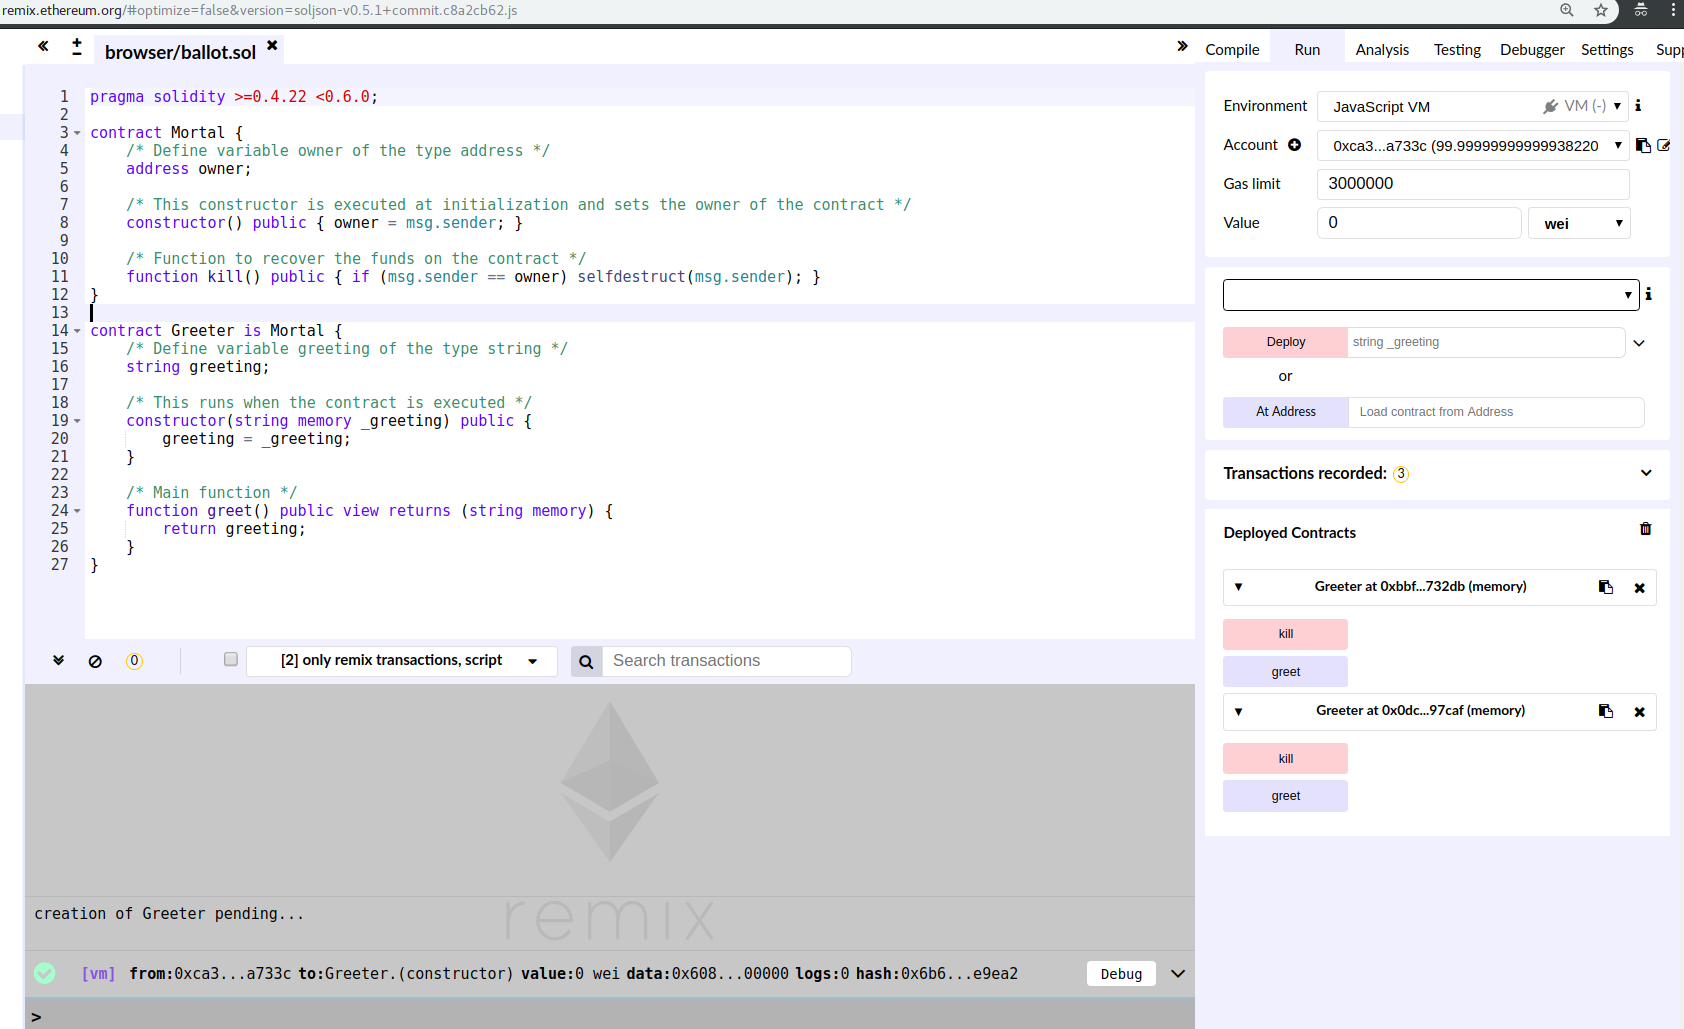
\includegraphics[width=0.8\textwidth]{contract-test}
\caption[contracttest]{Contrato sencillo con el único fin de probar Remix. (26)}
\label{fig:contract-test}
\end{figure}

\begin{figure}[htbp!] 
\centering    
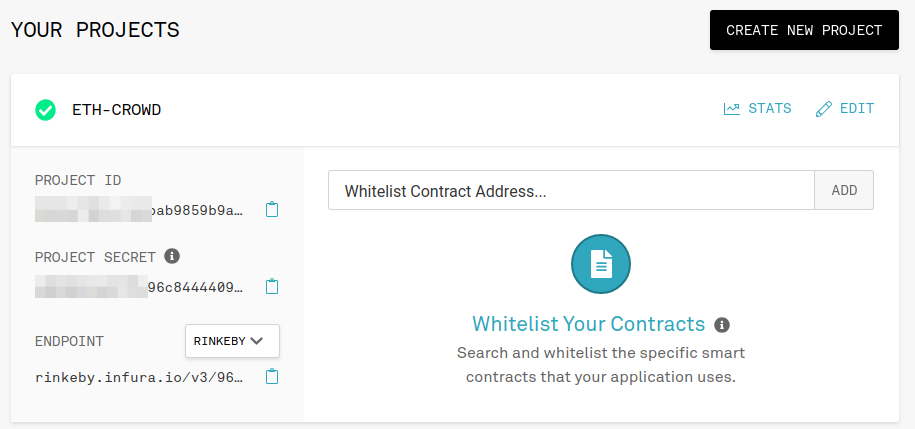
\includegraphics[width=0.8\textwidth]{infura-key}
\caption[infurakey]{Sección de la cuenta de Infura donde podemos obtener la access key. (27)}
\label{fig:infura-key}
\end{figure}

\subsection{Semana 6}
Se trabajó en el capítulo 2 del informe (17). Se creó el contrato Project en el IDE Remix
utilizando una versión de pragma solidity >=0.4.22 <0.6.0 y la versión de compilador
0.5.1+commit.c8a2cb62.Emscripten.clang (29). Se creó también el contrato ProjectBuilder con las 
mismas versiones utilizadas en el contrato Project (30).

En este punto del desarrollo debe decirse que ambos contratos compilan y se comportan correctamente
siendo utilizados en la plataforma Remix.

\subsection{Semana 7}
Durante esta semana se trabajó sobre los capítulos 1 y 2 del informe. Además, fue durante esta
semana donde comenzaron los problemas con las versiones de Node, Solidity, compiladores y librerías
utilizadas.

Como se dijo antes, durante la semana 6 se crearon los contratos Project y ProjectBuilder. Al 
comienzo de la semana 7 se comenzó la tarea de escribir un script de Node para poder compilar
los contratos con la librería \textit{solc v0.5.2} antes de deployarlos a la red (31). Luego de 
algunas horas investigando en la documentación de la librería y haciendo pruebas, logré compilar
lo que a simple vista parecía lo correcto para luego ser deployado a la red Rinkeby.

Teniendo el script compilando los contratos, se procedió a crear el script en Node para deployar
éstos a la red Rinkeby con la librería \textit{web3 v1.0.0-beta.38}. El script es sencillo, consta
de unas diez líneas de código pero sin embargo aquí es donde me topé con una pared de 
incompatibilidades. Detecté que el stack que la causaba eran las mencionadas versiones de 
\textit{solc} y \textit{web3} sumadas a Node v10. En los siguientes dos gráficos se puede ver
cómo el deploy entraba en un loop infinito contra la API de Infura, logrando llegar a más de mil
quinientos llamados al método \textit{eth\_getTransactionReceipt}. La llamada a este método es 
crucial debido a que en la respuesta (que nunca se pudo obtener correctamente) nos será devuelta
la dirección donde se deployó el contrato. Esta dirección le dirá luego a Node y React dónde tienen
que ir a buscar los métodos para ejecutar.

\begin{figure}[htbp!] 
\centering    
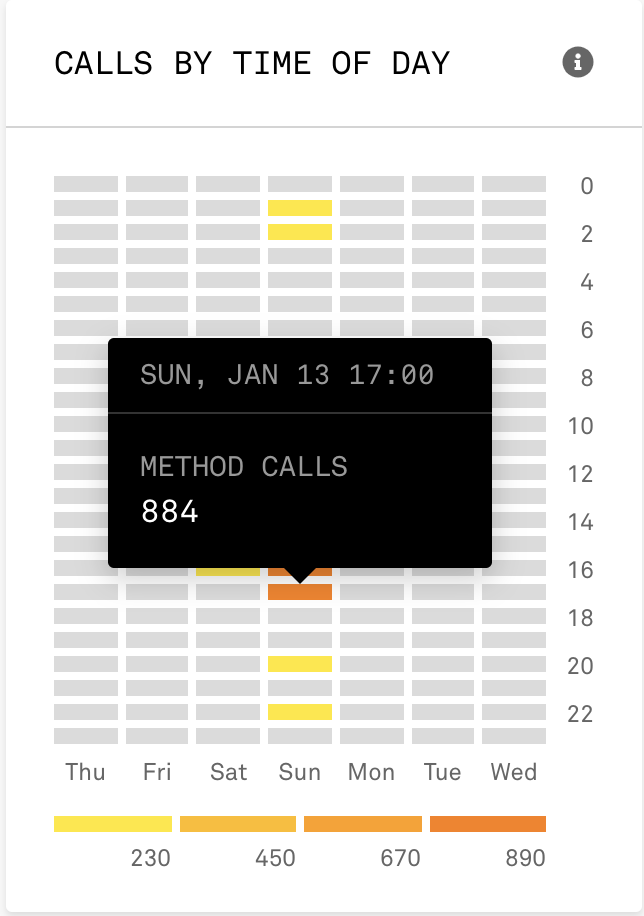
\includegraphics[width=0.8\textwidth]{infura-calls-1}
\caption[infuracalls1]{Se puede ver que entre las 16 y 17 horas (a la derecha) se produjeron un aproximado de 1760 llamados a la API de Infura.}
\label{fig:infura-calls-1}
\end{figure}

\begin{figure}[htbp!] 
\centering    
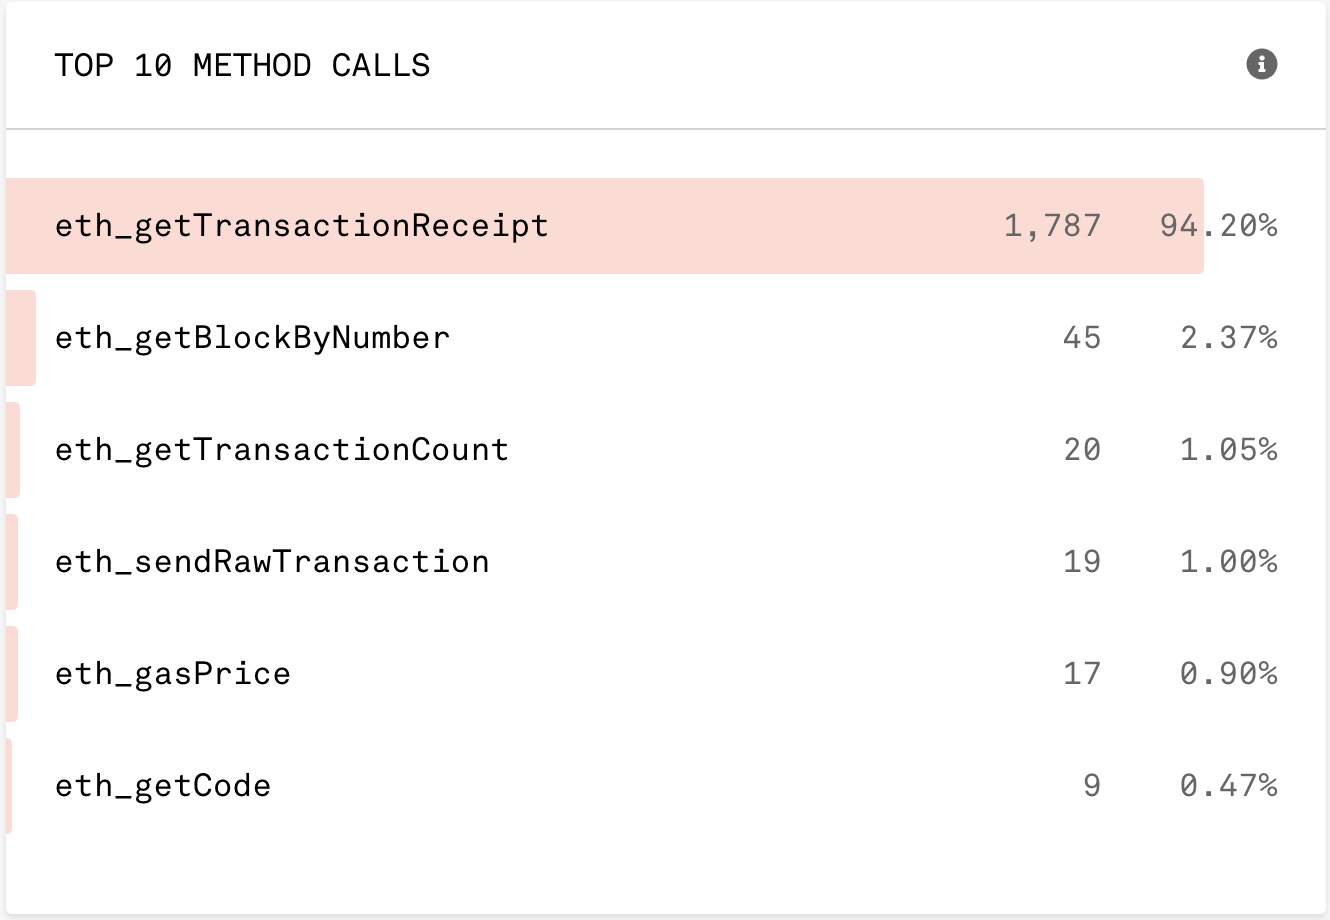
\includegraphics[width=0.8\textwidth]{infura-calls-2}
\caption[infuracalls2]{Se ve específicamente al método que se estaba llamando de la API.}
\label{fig:infura-calls-2}
\end{figure}

\begin{figure}[htbp!] 
\centering    
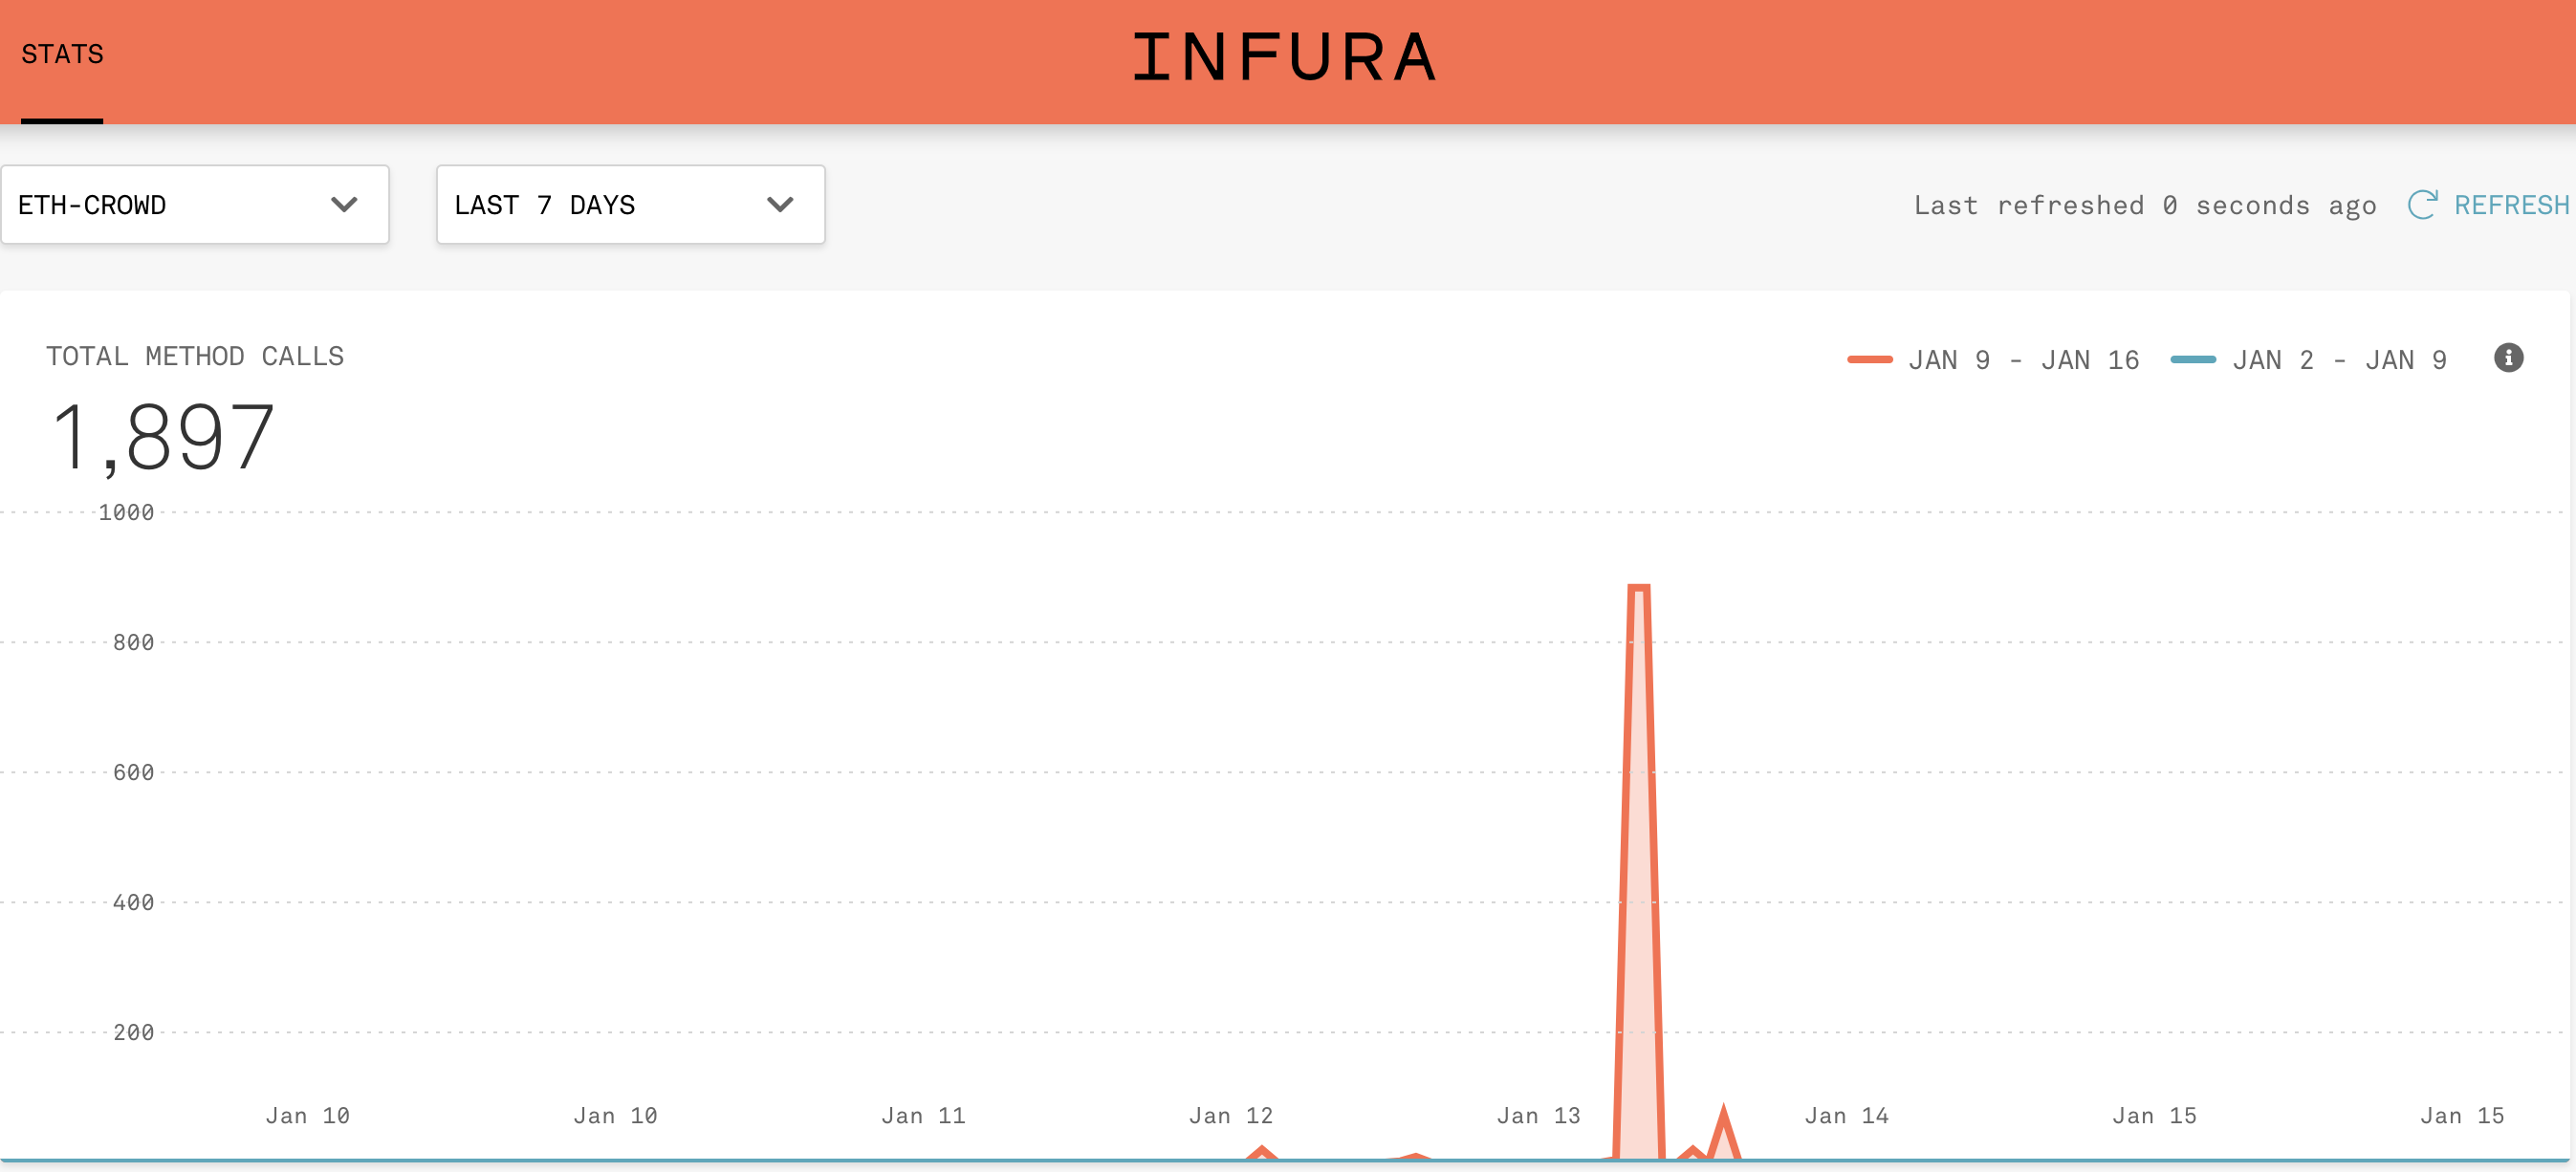
\includegraphics[width=0.8\textwidth]{infura-calls-3}
\caption[infuracalls3]{En el gráfico se ve el pico de actividad en la API cuando estaba sucediendo el bug del loop infinito.}
\label{fig:infura-calls-3}
\end{figure}


\subsection{Semana 8}
Durante esta semana se terminaron de escribir las primeras versiones de los capítulos 1 y 2
del informe y a su vez se comenzó a escribir el capítulo 3. Además, se hicieron diversas pruebas 
que llevaron más de 15 horas combinando versiones de Node, solc, web3, pragma solidity y del
compilador solidity para dar con la combinación definitiva para llevar adelante la app (28).

Las versiones finales que se encontraron 100\% compatibles y estables y que serán utilizadas para
todo el proyecto son:

\begin{itemize}
	\item Node v8.11.4
	\item Pragma Solidity \^0.4.17;
	\item Compiler (solo en Remix) 0.4.19+commit.c4cbbb05.Emscripten.clang
	\item Solc 0.4.19
	\item Web3 1.0.0-beta.26
\end{itemize}

\begin{figure}[htbp!] 
\centering    
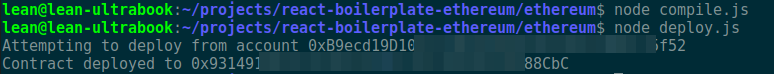
\includegraphics[width=0.9\textwidth]{success-deploy}
\caption[successdeploy]{Comandos para compilar y deployar funcionando correctamente. Se puede ver que cuando el contrato es deployado, se nos devuelve la dirección donde ha sido deployado.}
\label{fig:success-deploy}
\end{figure}

\subsection{Semana 9}
Teniendo seleccionadas las versiones estables del ecosistema de la app, se procedió a escribir
el código encargado de consumir los métodos de los contratos Project y ProjectBuilder (34).
Se escribió el código para conectarse a los contratos a través de web3 (35). Se probaron con éxito
las dos tareas previas.

Se hizo el set up completo del entorno front end con React, React Router, Webpack y Babel (36).

Se hicieron retoques en los capítulos 1 y 2 del informe y se continuó trabajando sobre el capítulo
3.

Se hizo el componente Index en React, el cual a través de web3 obtiene y muestra todos los
proyectos creados en la dirección que se le haya configurado (37).

\subsection{Semana 10}
Esta semana fue intensa en cuanto a desarrollo del front end, se investigó sobre buenas prácticas
en React y se pudieron hacer los componentes correspondientes a los tickets 39, 40, 41, 42, 43
y 44 (únicamente el HTML y Javascript, restando para la semana siguiente el CSS). En este punto
ya se puede decir que tenemos una aplicación completamente funcional, todos los componentes del 
front end desencadenan las acciones correspondientes para conectarse con los contratos y recibir
o enviar información. También el back end se encuentra completamente funcional, todos los comandos
creados funcionan correctamente. 

Se hicieron más retoques en los capítulos 1 y 2, también se añadieron imágenes.

Resta agregar los estilos a los componentes.

\subsection{Semana 11}
Durante esta semana se agregaron los estilos CSS a la aplicación, específicamente a los componentes
relacionados a los tickets 39, 40, 41, 42, 43 y 44. 

Se actualizó el capítulo 3 del informe hasta la semana 11 inclusive.


\subsection{...Semana N}